\documentclass[a4paper,11pt]{article}

%%%%%%%%%%%%%%%%%%% Packages %%%%%%%%%%%%%%%%%%%
\usepackage[utf8]{inputenc}
\usepackage[a4paper, margin=20mm, bindingoffset=0mm, heightrounded]{geometry}  % one of the few packages let you reconfigure (\geometry{})
\usepackage[backend=biber, style=alphabetic, sorting=ynt]{biblatex}
\usepackage[dvipsnames]{xcolor}  % for {Maroon}
\usepackage[british]{babel}  % for correct hyphenation
\usepackage{csquotes}
\usepackage{xhfill}  % for \xhrulefill
\usepackage[colorlinks=true,linkcolor=blue,filecolor=magenta,urlcolor=cyan,]{hyperref}
% \usepackage{ragged2e}  % for text alignment, but default \justify
\usepackage{tikz}
\usepackage{bm}

%%%%%%%%%%%%%%%%%%% Settings %%%%%%%%%%%%%%%%%%%
\setlength{\parindent}{0em}
\setlength{\parskip}{0.5em}

\addbibresource{bibliography/literature_review.bib}
\addbibresource{bibliography/references.bib}

\newcommand*\circled[1]{\tikz[baseline=(char.base)]{\node[shape=circle,draw,inner sep=2pt] (char) {#1};}}
            
%%%%%%%%%%%%%%%%%%% Document %%%%%%%%%%%%%%%%%%%
\title{Bio-image Segmentation and Classification}
\author{Qin Yu}
\date{April 2020}

\begin{document}
\maketitle
\tableofcontents

\section{Colours}
\begin{description}
    \item[Concepts don't understand yet] \xhrulefill{Maroon}{2pt}
\end{description}

\section{Image processing and cell tracking} 
Segment time-lapse movies of cells into foreground (cell) and background, a method in \textit{Local cellular neighbourhood controls proliferation in cell competition} \cite{bove2017local}.
\begin{description}
    \item[Restoration] (preprocessing) of the fluorescence images:
    \begin{enumerate}
        \item \textcolor{Maroon}{Flat-field illumination correction}
        \item \textcolor{Maroon}{Remove CCD ``hot pixel''}
    \end{enumerate}
    
    \item[Segmentation] using a \textcolor{Maroon}{Gaussian mixture model (GMM)}:
    \begin{enumerate}
        \item Take three images -- beginning, middle, end -- of the movie
        \item Fit these images to a GMM using \textcolor{Maroon}{expectation maximisation algorithm} \cite{xu1996convergence} to learn the appropriate parameter $\theta$
        \item Obtain \textcolor{Maroon}{intensity distribution} $P(x|\theta) = \sum^n_{k = 1}\lambda_k N_k (\bm{\mu}_k, \bm{\sigma}_k^2)$, where typically $n = 3$ and the three normal distribution reflect the intensity distributions of \textit{background}, \textit{interphase}, and \textit{mitotic}/\textit{apoptotic} cells (details of phases of the cell cycle see Fig. \ref{fig:cellcycle})
        \item Dense regions of cells where separated using either \textcolor{Maroon}{marker-controlled watershed transform}, or a hybrid of both methods
    \end{enumerate}
    
    \item[Merging/recombination] of over-segmented fragments of nuclei with a week fluorescence signal:
    \begin{enumerate}
        \item Calculate a Delaunay graph to make putative clusters of fragments
        \item Construct hypotheses for combinations of fragments \textcolor{Maroon}{constituting a single object}
        \item Assign equal prior probabilities to each hypotheses
        \item \textcolor{Maroon}{Perform successive Bayesian updates} using separation distance and image features
        \item Select the merging hypotheses with the highest posterior probabilities
    \end{enumerate}
    
    \item[Classification] of each nuclear marker into \textit{interphase}, \textit{pro(meta)phase}, \textit{metaphase}, \textit{anaphase}/\textit{telophase}, and \textit{apoptotic}.
    \begin{description}
        \item[CNN architecture] -- LeNet-5 \cite{lecun1998gradient,lecun2015lenet}: 
        \begin{enumerate}
            \item Several layers of $3\times3$ convolution, ReLU \cite{nair2010rectified}, and $2\times2$ max-pooling units \cite{scherer2010evaluation}, which decrease spatial dimensionality and increase the number of filters
            \item Several fully connected layers, which reduce the output to a one-dimensional tensor representing the five mutually exclusive cell cycle classes
            \item Final Softmax layer returns the output probabilities for each class
        \end{enumerate}
        \item[Deep CNN training] \mbox{}
        \begin{enumerate}
            \item Generate three data sets: 1) training, 2) test, 3) validation with equal size
            \item Augment the training examples by 1) rotations, 2) noise, 3) translations, to yield a large number of training examples
            \item Train using momentum optimiser with an exponentially decaying learning rate until convergence
            \item Measure accuracy by calculating a confusion matrix using the validation data set
        \end{enumerate}
    \end{description}
    
    \item[Assembly] of classified and segmented objects into tracks:
    \begin{description}
        \item[Assemble objects into tracklets (Def. \ref{def:tracklet}) \circled{?}] i.e. into reliable sections of track that do not contain cell division events:
        \begin{enumerate}
            \item The tracking algorithm assembles tracklets
            \item Each new tracklet initiates a probabilistic model in the form of a Kalman filter \cite{kalman1960new}
            \item Use this model to predict future states of each of the objects in the field of view
            \item Evaluate the posterior probability of each potential linkage from a Bayesian belief matrix for all possible linkage
            \item Assign new observations to the growing tracklet by this evaluation
            \item Correct errors using a temporal model of the cell cycle \cite{held2010cellcognition}
        \end{enumerate}
        \item[Assemble tracklets into lineage trees \circled{?}] by using multiple hypothesis testing and integer programming \cite{al2006automated,bise2011reliable} to identify a globally optimal solution:
        \begin{enumerate}
            \item 
        \end{enumerate}
    \end{description}
\end{description}

%%%%%%%%%%%%%%%%%%%%%%%%%%%%%%%%%%%%%%%%%%%%%%%%%%%%%%%%%%%%
\subsection{Details}
\subsubsection{Flat-field illumination correction}
\subsubsection{Charge-coupled device (CCD) and hot pixel}
\subsubsection{Gaussian mixture model (GMM)}
To understand Gaussian mixture model, one had better understand the K-means algorithm:
\begin{description}
    \item[K-means:] (hard EM)
    \begin{enumerate}
        \item set $k$ random centres, i.e. means, of clusters
        \item use the least squared Euclidean distance to assign each data point to the nearest mean. i.e. partitioning the observations according to the Voronoi diagram generated by the means
        \item update the centres' coordinates. i.e. recalculate means/centroids for observations assigned to each cluster
    \end{enumerate}

    \item[Gaussian Mixture Model (GMM)] (stochastic EM):
    \begin{itemize}
        \item Clusters modelled as Gaussians, not just their mean
        \item Assign data to clusters with some probability 
        \item Gives probability model of x (generative)
    \end{itemize}
\end{description}
Reference: \href{https://youtu.be/qMTuMa86NzU}{Gaussian Mixture Models and EM by Alexander Ihler}

\begin{description}
    \item[Python Packages] required
    \begin{itemize}
        \item \texttt{numpy}
        \item \texttt{cv2}
        \item \texttt{sklearn.mixture.GaussianMixture}
    \end{itemize}
\end{description}
Reference: \href{https://youtu.be/kkAirywakmk}{What is GMM and how to use it for Image segmentation? by Sreeni}\\

\begin{description}
    \item[Fuzzy image segmentation:] In image processing and computer vision, traditional image segmentation models often assign to one pixel only one exclusive pattern. In fuzzy or soft segmentation, any pattern can have certain ``ownership'' over any single pixel. If the patterns are Gaussian, fuzzy segmentation naturally results in Gaussian mixtures. Combined with other analytic or geometric tools (e.g., phase transitions over diffusive boundaries), such spatially regularised mixture models could lead to more realistic and computationally efficient segmentation methods.
\end{description}
Reference: \href{https://en.wikipedia.org/wiki/Mixture_model\#Fuzzy_image_segmentation}{Fuzzy image segmentation - Wikipedia}

More intuition and coding: \href{https://youtu.be/JNlEIEwe-Cg}{Gaussian Mixture Models by Siraj Raval}


\section{Definitions}
\subsection{Tracklet}
\label{def:tracklet}
Yes you guessed it right, tracklet is basically a short track between 5 or 6 frames generally. Track generally refers to the entire trajectory of a unique object's (person) path. During training, we give short paths of different individuals referred to as tracklet. AFAIK, short paths are chosen because most tracking algorithms use a constant velocity linear motion model - and short tracks are usually straight lines and change is velocity is very small.

The term is very informal, as I couldn't find any literature about it as well when I was working on a tracking problem.

Reference: \href{https://stackoverflow.com/questions/55512548/whats-the-difference-between-track-and-tracklet-in-tracking}{What's the difference between track and tracklet in tracking?}

\subsection{Phases of the cell cycle}
\begin{figure}[!htb]
    \centering
    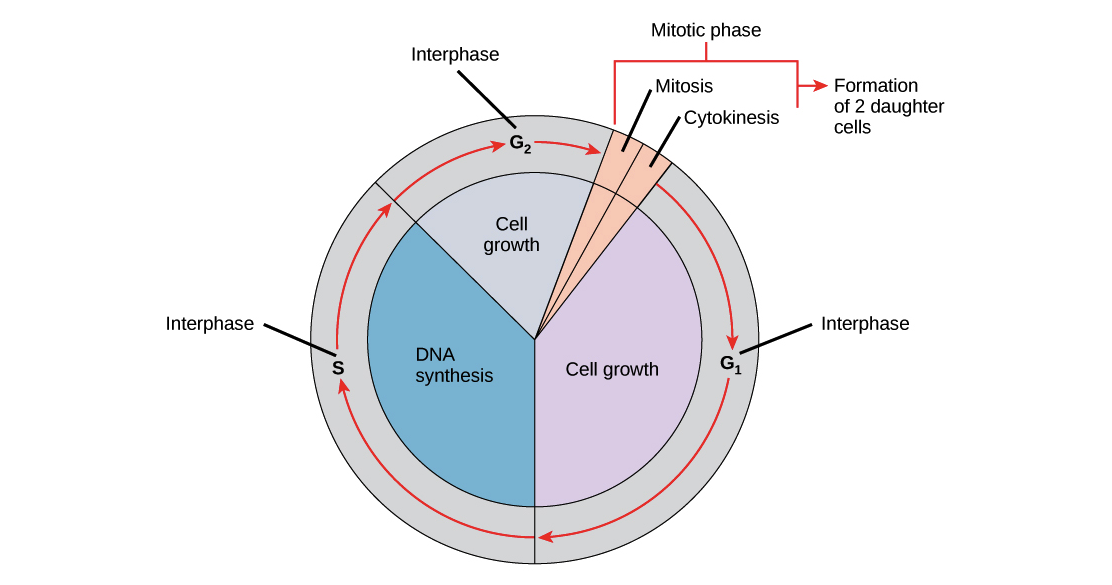
\includegraphics[width=\textwidth]{figures/cell_cycle.png}
    \caption{The cell cycle consists of interphase and the mitotic phase. During interphase, the cell grows and the nuclear DNA is duplicated. Interphase is followed by the mitotic phase. During the mitotic phase, the duplicated chromosomes are segregated and distributed into daughter nuclei. The cytoplasm is usually divided as well, resulting in two daughter cells.}
    \label{fig:cellcycle}
\end{figure}
Reference: \href{https://www.khanacademy.org/science/biology/cellular-molecular-biology/mitosis/a/cell-cycle-phases}{Phases of the cell cycle}, \href{http://cnx.org/contents/185cbf87-c72e-48f5-b51e-f14f21b5eabd@9.87:52/The-Cell-Cycle}{The Cell Cycle}

\section{Timeline}
\label{sec:timeline}

\begin{description}
    \item[30 Mar 2020] \mbox{}
    \begin{enumerate}
        \item Received documents from Alexis
        \item Skimmed through \textit{CRUK proposal}, focused on Aim 3.
        \item Read \textit{Explanation of data}
    \end{enumerate}
    
    \item[31 Mar 2020] \mbox{}
    \begin{enumerate}
        \item Meeting with Alexis and Andre
        \item Installed Fiji
        \item Read \cite{bove2017local}
    \end{enumerate}

    \item[1 Apr 2020] \mbox{}
    \begin{enumerate}
        \item Meeting with Tom
        \item Read \cite{bove2017local}
    \end{enumerate}
    
    \item[2 Apr 2020] \mbox{}
    \begin{enumerate}
        \item Summarised \cite{bove2017local} \textit{Local cellular neighbourhood controls proliferation in cell competition}
        \item Installed Mathematica
        \item \href{https://gist.github.com/qin-yu/d3619a68d209dd1feefd7385e43c3fc4}{Installed TensorFlow with GPU support}
    \end{enumerate}
\end{description}


\printbibliography

\end{document}
